\documentclass[format=acmsmall, review=false, screen=true]{acmart}

\usepackage{booktabs} % For formal tables

\usepackage[ruled]{algorithm2e} % For algorithms
\renewcommand{\algorithmcfname}{ALGORITHM}
\SetAlFnt{\small}
\SetAlCapFnt{\small}
\SetAlCapNameFnt{\small}
\SetAlCapHSkip{0pt}
\IncMargin{-\parindent}

\usepackage[T1]{fontenc}
\usepackage{ae,aecompl}
\usepackage{times}
\usepackage{graphicx}
\usepackage{caption}

\DeclareCaptionSubType*[arabic]{figure}
\captionsetup[subfigure]{labelformat=simple,labelsep=colon}

% correct bad hyphenation here
\hyphenation{op-tical net-works semi-conduc-tor In-ter-ac-tive 
On-de-mand Con-ser-va-tive}

% custom commands
\newcommand\todo[1]{\textcolor{red}{TODO\xspace#1}}
\newcommand\FIXME[1]{\textcolor{red}{FIX:}\textcolor{red}{#1}}
\newcommand\pubauthor[1]{\textit{#1}\xspace}
\newcommand\fname[1]{\textit{#1}\xspace}
\newcommand\fabbr[1]{\uppercase{#1}\xspace}

% NAMES
\newcommand\Android{\fname{Android}}

% ABBREVIATIONS
\newcommand\Cpu{\fabbr{Cpu}}
\newcommand\Dvfs{\fabbr{Dvfs}}

% OTHER
\newcommand\Ondemand{\texttt{Ondemand}\xspace}
\newcommand\Interactive{\texttt{Interactive}\xspace}
\newcommand\Conservative{\texttt{Conservative}\xspace}


%-------------------Results and Numbers----------------------------------
\newcommand\totalinputevents{1935\xspace} % total input events (including spurious, noisy, tap and swipes)
\newcommand\totalinputeventsRN{1852\xspace}
\newcommand\totalswipes{4\%\xspace} % percentage of swipe input events
\newcommand\totalspurious{1\%\xspace} % percentage of spurious input events



% Metadata Information
\acmJournal{TACO}
%\acmVolume{9}
%\acmNumber{4}
%\acmArticle{39}
%\acmYear{2010}
%\acmMonth{3}
%\copyrightyear{2009}
%\acmArticleSeq{9}

% Copyright
%\setcopyright{acmcopyright}
\setcopyright{acmlicensed}
%\setcopyright{rightsretained}
%\setcopyright{usgov}
%\setcopyright{usgovmixed}
%\setcopyright{cagov}
%\setcopyright{cagovmixed}

% DOI
%~ \acmDOI{0000001.0000001}

% Paper history
%~ \received{February 2007}
%~ \received[revised]{March 2009}
%~ \received[accepted]{June 2009}

\begin{document}

\title[Awesome]
{My Awesome Publication}

\author{Volker Seeker}
\author{Peter BlaBla}
\affiliation{%
  \institution{University of Edinburgh}
  \streetaddress{Informatics Forum, 10 Crichton Street}
  \city{Edinburgh}
  %\state{VA}
  \postcode{EH8 9AB}
  \country{United Kingdom}
}

\begin{abstract}
    
This is a great paper. You should cite it.

\end{abstract}



%
% The code below should be generated by the tool at
% http://dl.acm.org/ccs.cfm
% Please copy and paste the code instead of the example below.
%
\begin{CCSXML}
<ccs2012>
 <concept>
  <concept_id>10010520.10010553.10010562</concept_id>
  <concept_desc>Computer systems organization~Embedded systems</concept_desc>
  <concept_significance>500</concept_significance>
 </concept>
 <concept>
  <concept_id>10010520.10010575.10010755</concept_id>
  <concept_desc>Computer systems organization~Redundancy</concept_desc>
  <concept_significance>300</concept_significance>
 </concept>
 <concept>
  <concept_id>10010520.10010553.10010554</concept_id>
  <concept_desc>Computer systems organization~Robotics</concept_desc>
  <concept_significance>100</concept_significance>
 </concept>
 <concept>
  <concept_id>10003033.10003083.10003095</concept_id>
  <concept_desc>Networks~Network reliability</concept_desc>
  <concept_significance>100</concept_significance>
 </concept>
</ccs2012>
\end{CCSXML}

\ccsdesc[500]{Computer systems organization~Embedded systems}
\ccsdesc[300]{Computer systems organization~Redundancy}
\ccsdesc{Computer systems organization~Robotics}
\ccsdesc[100]{Networks~Network reliability}

%
% End generated code
%

\keywords{Wireless sensor networks, media access control,
multi-channel, radio interference, time synchronization}


%~ TODO kudos to the grant?
%~ This work was supported by the National Natural Science Foundation of China under Grant No. 61502450,
%~ Grant No. 61432018, Grant No. 61521092, and Grant No. 61272136; National Key Research and Development
%~ Program of China under Grant No.2016YFB0200803; NSF project 1216569; and a gift fund from AMD Inc.
%~ 
\thanks{Thanks for all the hard work. This is awesome.}

\maketitle

\renewcommand{\shortauthors}{V. Seeker et. al.}

\section{Introduction}
\label{sec:introduction}

This is an introduction.

\paragraph{Contributions} This paper makes the following specific contributions:

\begin{enumerate}
\item great contribution
\item fantastic contribution
\end{enumerate}

\paragraph{Overview}
The remainder of this paper is structured as follows. We motivate 
our work in Section~\ref{sec:motivation}. In Section~\ref 
{sec:methodology} we present our novel approach. This is followed in 
Section~\ref{setup} by a description of our experimental setup. 
A presentation of 
experimental results can be found in Section~\ref{results}. We 
discuss related work in Section~\ref{relatedwork} before we 
summarise and conclude in Section~\ref{sec:summary}.

\section{Motivation}
\label{sec:motivation}

Figure~\ref{fig:motivation} shows a short snapshot of how the
frequency of the \Cpu adapts to four input events for two different
\Dvfs governors. WOW so motivating.

%% FIGURE: Workload Snapshot -------------------------------------------------
\begin{figure}[t!]
  \begin{centering}
    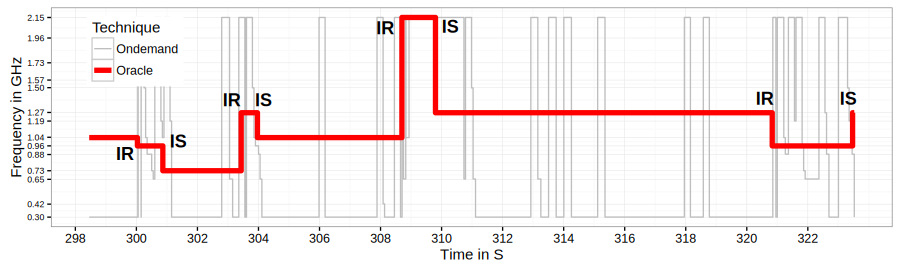
\includegraphics[width=1\columnwidth]{figures/motivation}
    \par
  \end{centering}
  \caption{Snapshot of the behavior of the \Ondemand governor and
	  another more energy efficient governor for one of this study's
	  interactive workloads. \textbf{IR} indicates when user input was
	  received and \textbf{IS} indicates the earliest time when the user
	  would perceive the input as serviced.
  \label{fig:motivation}}
\end{figure}
% ------------------------------------------------------------------------------


\section{Methodology}
\label{sec:methodology}

This methodology is particularly novel.

\section{Experimental Setup and Execution}
\label{setup}

What a clever setup this is.

\section{Experimental Results}
\label{results}

These results are breathtaking.

\section{Related Work}
\label{relatedwork}

This paper~\cite{seeker2014measuring} by \pubauthor{Seeker~et~al} is great, you should
cite it too.


\section{Conclusions and Future Work}
\label{sec:summary}

Everything is summarised so clearly.


% Bibliography
\bibliographystyle{../lib/ACM-Reference-Format}
\bibliography{main}

\end{document}
